% Copyright (C) 2015 Chen-Pang He <http://jdh8.org/>
%
% This file may be distributed and/or modified under
%
% 1. LaTeX Project Public License
% 2. GNU Public License
%
% See the files COPYING.* for more details.

\documentclass{Slideshow}
\newcommand{\mmhref}[2]{\href{http://us.metamath.org/mpeuni/#1.html}{#2}}

\begin{document}
\title[微積分演習課]{臺北醫學大學微積分演習課}
\maketitle

\section{前言}
\subsection{關於}
\begin{frame}{關於我}
    \begin{columns}[onlytextwidth]
        \begin{column}{0.6\textwidth}
            \begin{itemize}
                \item \href{http://my2.tmu.edu.tw/b101100025}{B101100025}
                \item \href{https://www.facebook.com/jdh863}{臉書}
                \item \href{https://plus.google.com/+\%E4\%BD\%95\%E9\%9C\%87\%E9\%82\%A6-jdh8}{Google+}
                \item 0918-319823
                    \begin{itemize}
                        \item 真是充滿火藥味的號碼
                    \end{itemize}
            \end{itemize}
        \end{column}

        \begin{column}{0.4\textwidth}
            \begin{flushleft}
                \newlength{\stickerwidth}
                \setlength{\stickerwidth}{\columnwidth - 1em}
                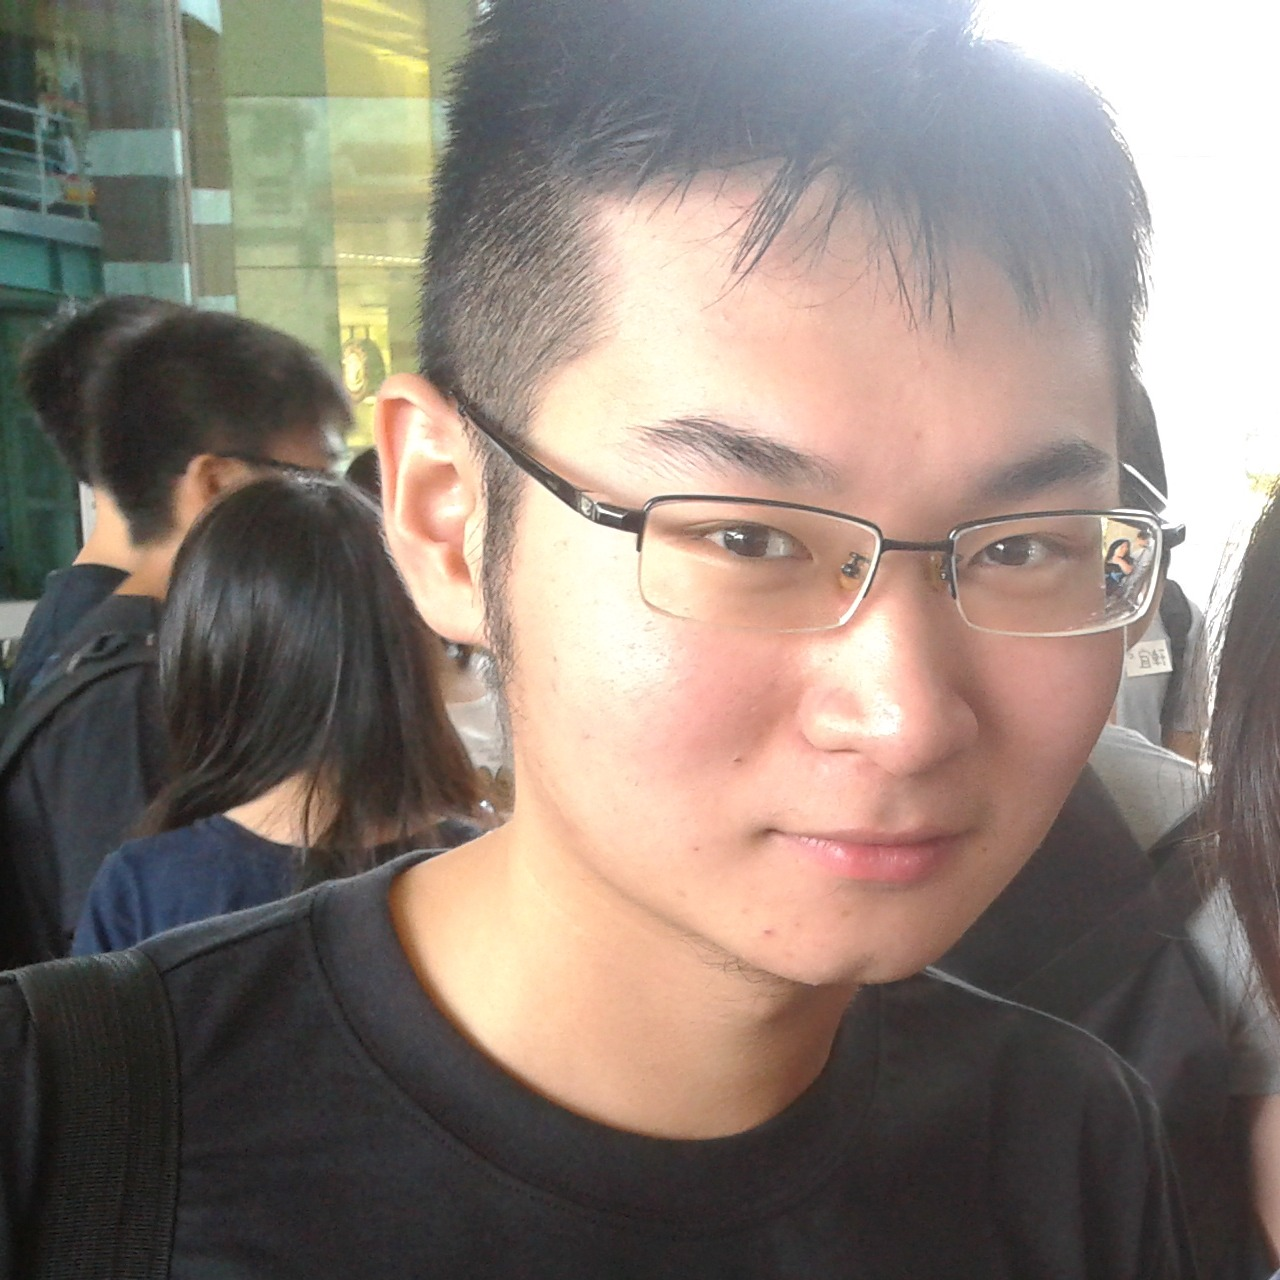
\includegraphics[width=\stickerwidth]{Introduction/sticker.jpg}
            \end{flushleft}
        \end{column}
    \end{columns}
\end{frame}

\begin{frame}{課程內容}
    以培養解題能力為目標。先通過考試,後培養邏輯思辨能力。

    \begin{itemize}
        \item \href{https://jdh8.github.io/calculus-slides/}{投影片}
        \item \href{http://jdh8.org/category/calculus-course/}{考古題、上課影片}
        \item 網頁教材(建構中)
            \begin{itemize}
                \item \href{http://jdh8.org/calculus/}{部落格頁面}
                \item \href{https://zh.wikibooks.org/wiki/\%E5\%BE\%AE\%E7\%A7\%AF\%E5\%88\%86\%E5\%AD\%A6}{維基教科書}
            \end{itemize}
    \end{itemize}
\end{frame}

\begin{frame}{Copyleft}
    本系列教材具有圖文創作與程式創作的性質,所以同時以下列條款釋出。

    \begin{description}
        \item[CC BY-SA] 適合圖文創作
        \item[GPL\scriptsize~v3+] 適合程式創作
    \end{description}

    Copyleft 允許閱聽人自由使用、複製、研究、修改著作,但必須以相同方式分享。

    \begin{figure}
        \href
            {https://commons.wikimedia.org/wiki/File:Copyleft.svg}
            {
\includegraphics[width=5em]{Introduction/Copyleft.pdf}}
    \end{figure}
\end{frame}

\subsection{微積分是什麼}
\begin{frame}{先備知識}
    \begin{figure}
        \href
            {https://commons.wikimedia.org/wiki/File:Japanese_Senbeis.jpg}
            {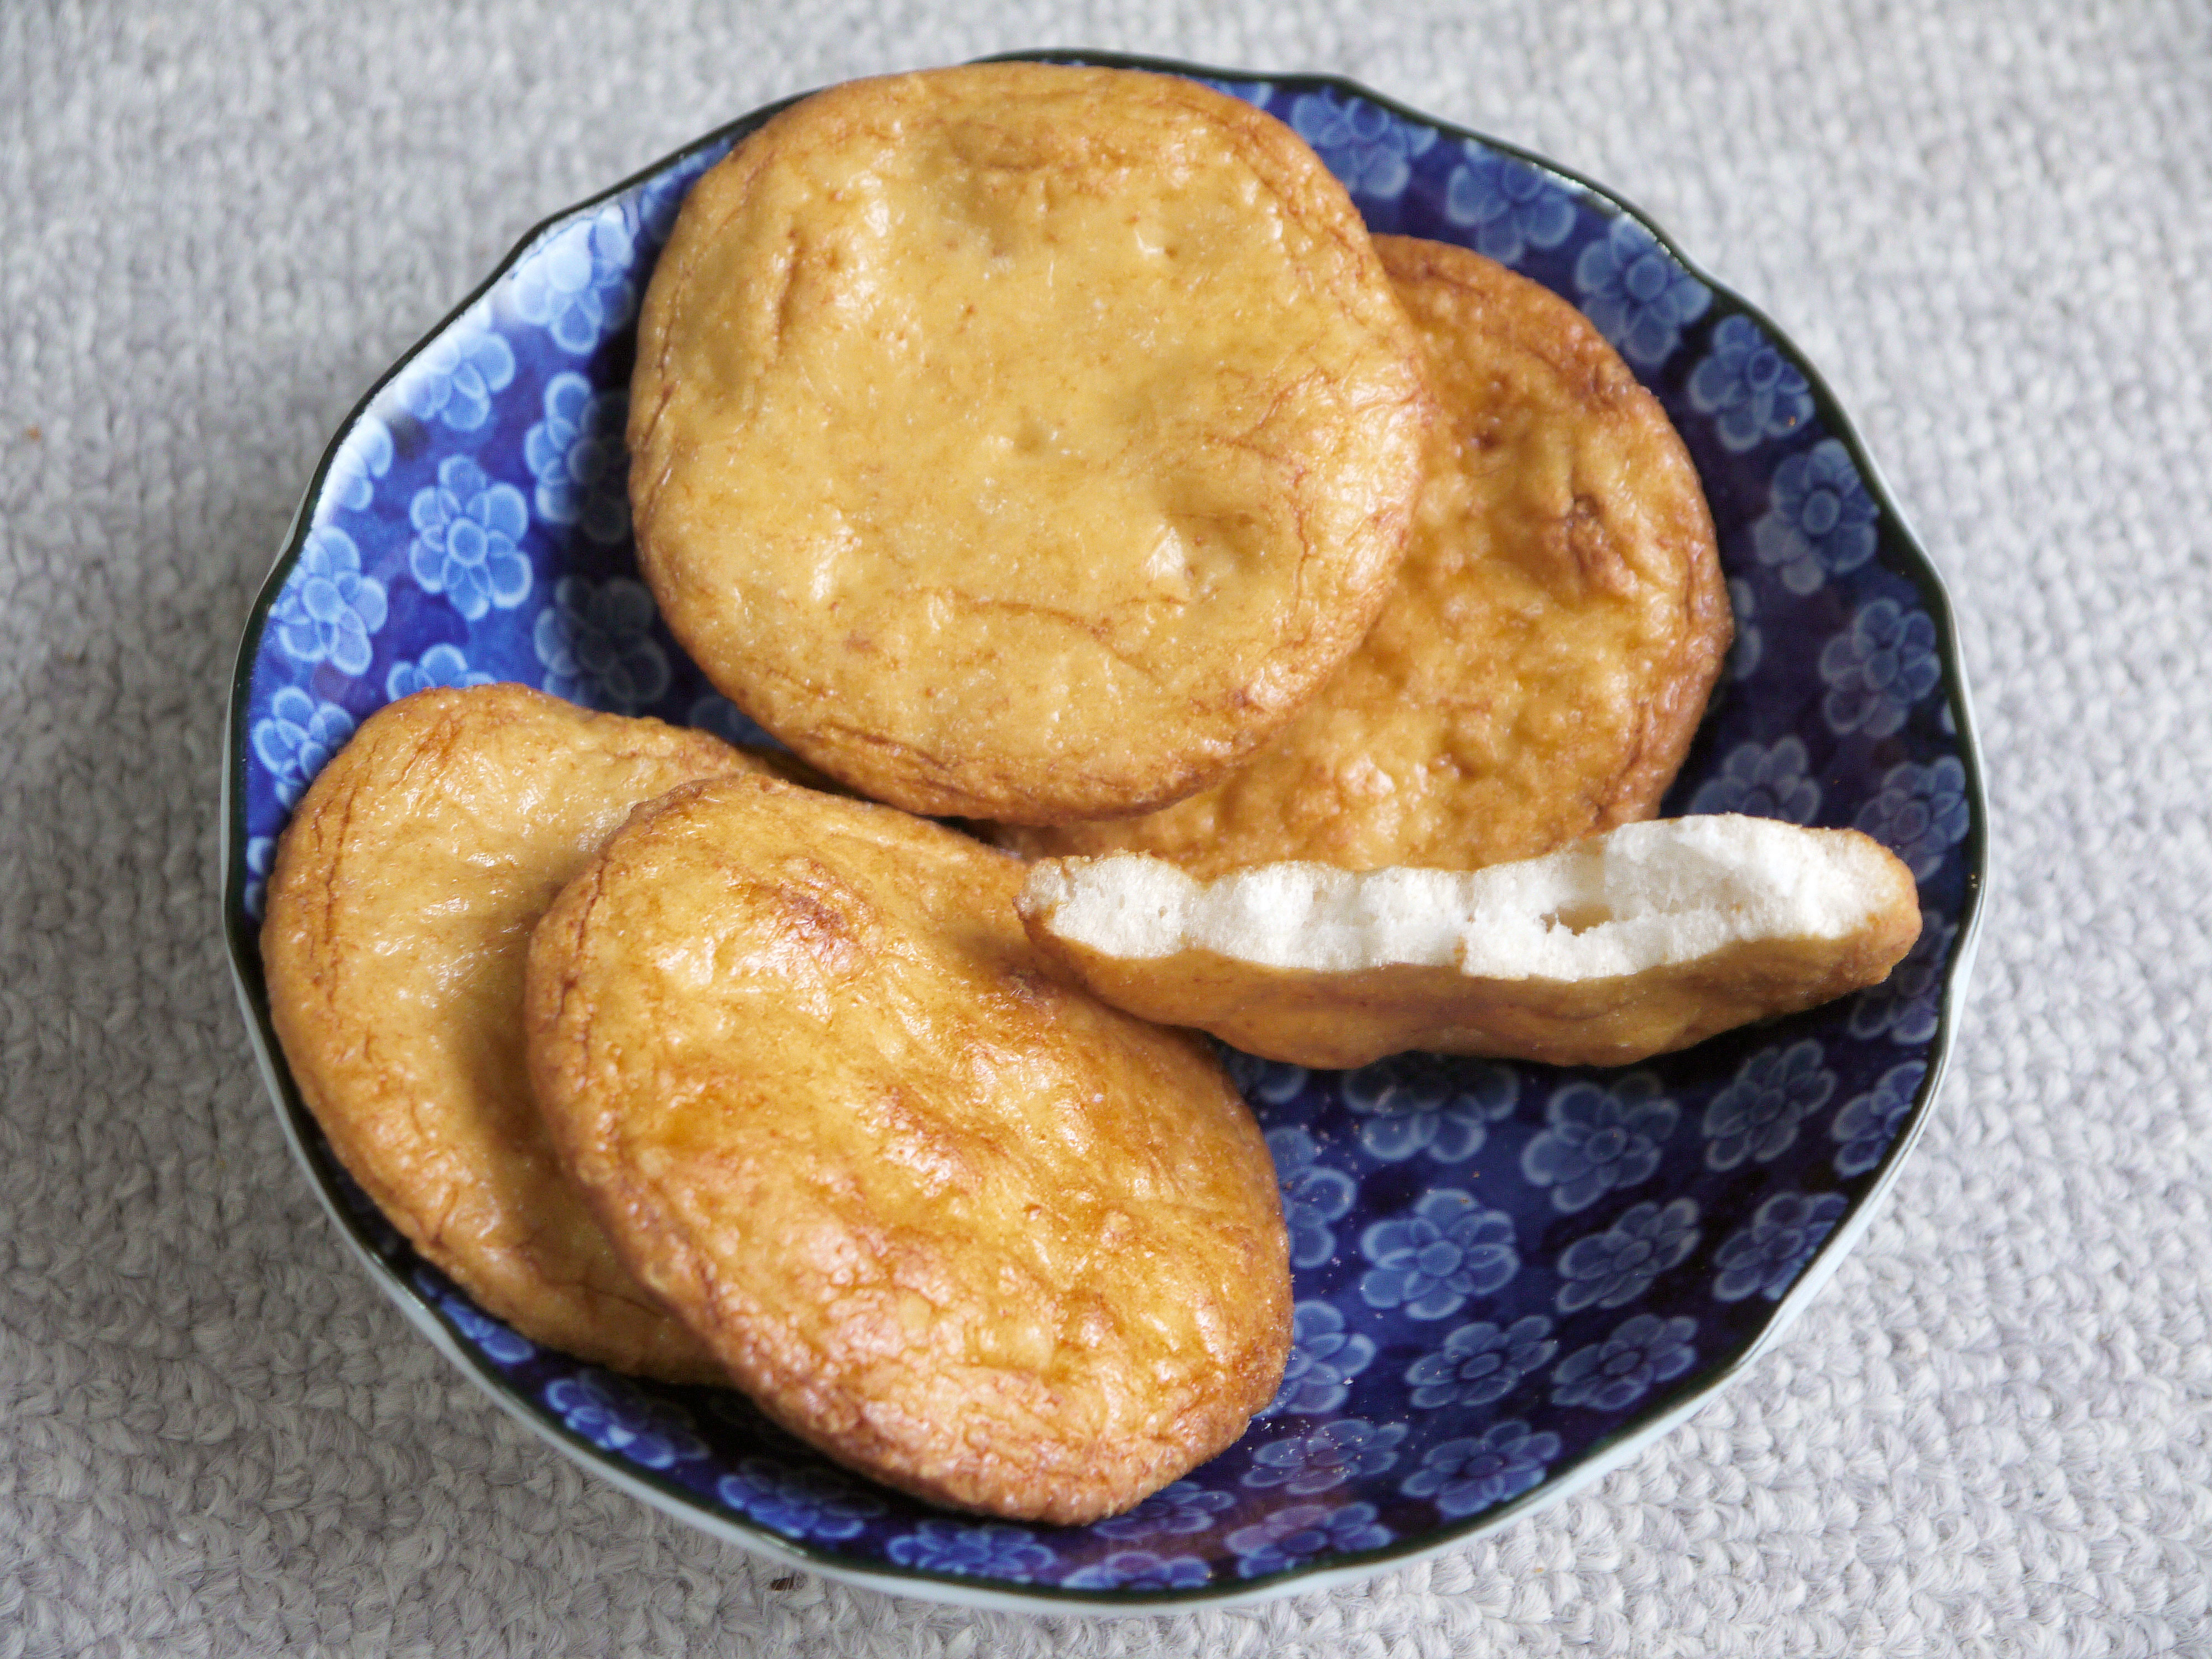
\includegraphics[width=\textheight]{Introduction/Japanese_Senbeis.jpg}}
        \caption{\href{https://ja.wikipedia.org/wiki/\%E7\%85\%8E\%E9\%A4\%85}{仙貝},由 DryPot 所攝}
    \end{figure}
\end{frame}

\begin{frame}
    \begin{quote}
        If people do not believe that mathematics is simple, it is only because
        they do not realize how complicated life is.

        \begin{flushright}
            \textup{John von Neumann (1903--1957)}
        \end{flushright}
    \end{quote}
\end{frame}

\begin{frame}{微積分是什麼}
    微積分是研究\textbf{連續}、\textbf{變化}的數學。

    \begin{description}
        \item[連續] 用\textbf{實數}來表示連續
        \item[變化] 用\textbf{函數}來表示變化
    \end{description}

    微積分的主要研究對象是以實數為參數的函數。
\end{frame}

\section{集合}
\begin{frame}{集合}
    數學是研究\textbf{數}和\textbf{形}的學問。數學家發現他們都可以用\textbf{集合}來表示。

    數學的宇宙就是\href
        {https://zh.wikipedia.org/wiki/\%E5\%86\%AF\%C2\%B7\%E8\%AF\%BA\%E4\%BC\%8A\%E6\%9B\%BC\%E5\%85\%A8\%E9\%9B\%86}
        {集合的宇宙}。

    \begin{itemize}
        \item 集合可以等於其他集合
        \item 集合內只有集合
        \item 集合一定屬於另一個集合
    \end{itemize}

    集合可以透過公理化集合論定義。
    \mmhref{mmtheorems}{Metamath} 有精美範例。
\end{frame}

\begin{frame}{無序對}
    \begin{definition}
        \newcommand{\thepair}{\left\{ A, B \right\}}
        \mmhref{ax-pr}{配對公理}讓我們可以從兩集合 $A$, $B$ 建構出新的集合
        \[ \thepair \]
        使得 $x \in \thepair$ 就是指 $x = A$ 或 $x = B$。
    \end{definition}

    如果 $A = B$ 就變成了 $\left\{ A, A \right\}$ 可以進一步簡寫為
    \[ \left\{ A \right\}.\]
\end{frame}

\begin{frame}{序對}
    \begin{definition}
        為了確保 $\left\langle A, B \right\rangle = \left\langle C, D \right\rangle$ 意同
        \[ A = C \quad \mbox{且} \quad B = D,\]

        可以定義
        \begin{equation}
            \left\langle A, B \right\rangle =
            \left\{ \left\{ A \right\}, \left\{ A, B \right\} \right\}.
            \label{eq:df-op}
        \end{equation}
    \end{definition}

    \eqref{eq:df-op} 不是從集合定義序對的唯一方法。
\end{frame}

\subsection{關係與函數}
\begin{frame}{關係}
    \begin{definition}
        一般我們把 $A$, $B$, $R$ 三個集合寫在一起的句子
        \[ ARB \]

        視為 $\left\langle A, B \right\rangle \in R$ 的簡寫。
    \end{definition}

    \begin{example}
        \[ 1 < 2 \quad \mbox{即} \quad \left\langle 1, 2 \right\rangle \in\ < .\]
    \end{example}
\end{frame}

\begin{frame}{反關係}
    \begin{definition}
        反關係就是把關係的左右參數互換。
        \[ A R^{-1} B \quad \mbox{即} \quad BRA.\]
    \end{definition}

    \begin{example}
        \[ > \ = \ <^{-1}.\]
    \end{example}
\end{frame}

\begin{frame}{複合關係}
    \begin{definition}
        滿足複合關係,意味著存在著「中間人」串起兩個關係。

        \[ A \left( F \circ G \right) B \]

        即存在一個 $x$ 使得
        \[ AGx \quad \mbox{且} \quad xFB \]
    \end{definition}

    \begin{example}
        \[ \mbox{姑姑} = \left( \mbox{姐妹} \circ \mbox{爸爸} \right). \]
    \end{example}
\end{frame}
\end{document}
